\documentclass[tikz]{standalone}

% \usepackage{tikz}
\usetikzlibrary{trees}

\begin{document}

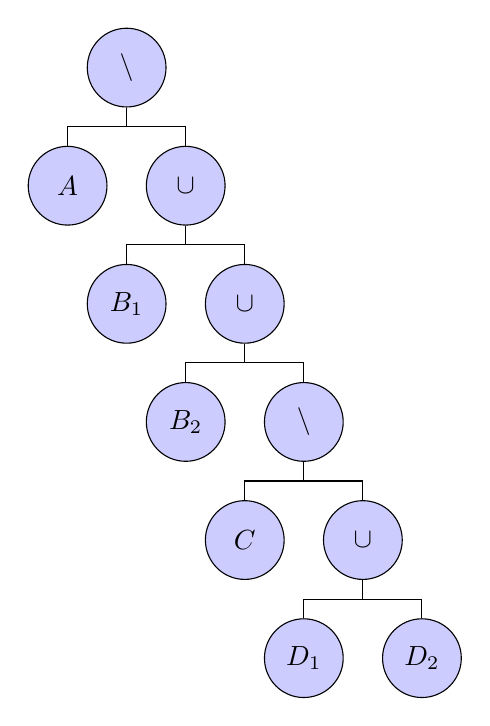
\begin{tikzpicture}[
mystyle/.style={draw, circle, minimum size = 1cm, fill = blue!20},
edge from parent fork down
]
\node[mystyle] {$\setminus$}
    child {node[mystyle] {$A$}}
    child {node[mystyle] {$\cup$}
    	child {node[mystyle] {$B_1$}}
    	child {node[mystyle] {$\cup$}
    		child {node[mystyle] {$B_2$}}
    		child {node[mystyle] {$\setminus$}
    			child {node[mystyle] {$C$}}
    			child {node[mystyle] {$\cup$}
    				child {node[mystyle] {$D_1$}}
    				child {node[mystyle] {$D_2$}}
    			}
    		}
    	}
    };
\end{tikzpicture}

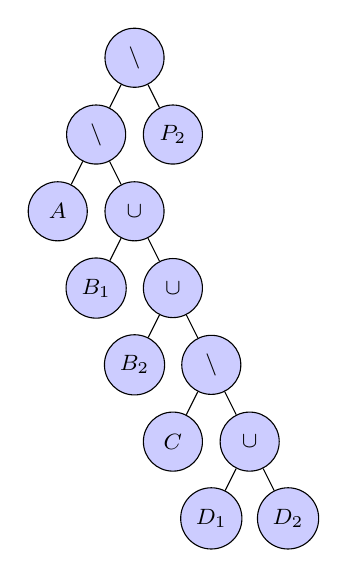
\begin{tikzpicture}[
mystyle/.style={draw, circle, minimum size = 0.75cm, fill = blue!20, font = \footnotesize},
scale=0.65
]
\node[mystyle] {$\setminus$}
	child {node[mystyle] {$\setminus$}
		child {node[mystyle] {$A$}}
		child {node[mystyle] {$\cup$}
    	   child {node[mystyle] {$B_1$}}
    	   child {node[mystyle] {$\cup$}
    	   	   child {node[mystyle] {$B_2$}}
    	   	   child {node[mystyle] {$\setminus$}
    	   	   	   child {node[mystyle] {$C$}}
    	   	   	   child {node[mystyle] {$\cup$}
    	   	   	   	   child {node[mystyle] {$D_1$}}
    	   	   	   	   child {node[mystyle] {$D_2$}}
    	   	   	   }
    	   	   }
    	   }
        }
	}
    child {node[mystyle] {$P_2$}};
\end{tikzpicture}

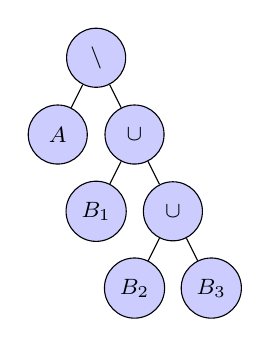
\begin{tikzpicture}[
mystyle/.style={draw, circle, minimum size = 0.75cm, fill = blue!20, font = \footnotesize},
scale=0.65
]
\node[mystyle] {$\setminus$}
        child {node[mystyle] {$A$}}
        child {node[mystyle] {$\cup$}
           child {node[mystyle] {$B_1$}}
           child {node[mystyle] {$\cup$}
               child {node[mystyle] {$B_2$}}
               child {node[mystyle] {$B_3$}
               }
           }
        };
\end{tikzpicture}

\end{document}